\documentclass{beamer}
\usepackage{appendixnumberbeamer}
\usepackage[ngerman]{babel}
\usetheme[progressbar=frametitle]{metropolis}

\title{Einstieg in die Untersuchung der Erklärbarkeit von Objektklassifikation auf ML-Basis am Beispiel eines Barcode-Detektors}
\date{\today}
\author{Semih Kasap}
\institute{Institut der Pathologie, Charité Berlin\newline 
Hochschule für Technik und Wirtschaft Berlin}
\begin{document}
  \maketitle
  \begin{frame}{Überblick}
    \begin{itemize}
      \item Vertrauen %TODO: prüfen, ob ich was zur Erklärbarkeit finde und ggf. diesen Abschnitt umbenennen zu "Erklärbarkeit"
%      \item Forschung, Gesellschaft und Politik %TODO: notwendig?
      \item Ansätze
      \item Werkzeuge
      \item Anwendung auf den Barcode-Detektor
    \end{itemize}
  \end{frame}

  \section{Vertrauen}

  \begin{frame}{Warum das Ganze?}
    \textbf{Sorge}: Wenn der Anwender einem KI-Modell nicht vertraut, wird dieser es nicht nutzen.
  \end{frame}

  \begin{frame}{Vertrauen I}
    \textbf{Vertrauen}, emotionale Sicherheit, einem anderen Menschen und dem eigenen Dasein offen gegenübertreten und sich hingeben zu können(...).
    
    Brockhaus, Vertrauen. http://brockhaus.de/ecs/enzy/article/vertrauen (aufgerufen am 2020-04-28)
   \end{frame}

  \begin{frame}{Vertrauen II}
    \textbf{im KI-Kontext:}
    \begin{enumerate}
      \item Einer \textbf{Vorhersage} vertrauen (z. B., ob der Anwender einer individuellen Vorhersage vertraut, um auf dieser Grundlage Aktionen zu tätigen)
      \item Einem \textbf{Modell} vertrauen (z. B., ob der Anwender sein Verhalten nachvollziehbar auf Grundlage seines Vertrauens in ein KI-Modells tätigt, nachdem das Modell für den Produktiveinsatz freigegeben wurde)
    \end{enumerate}
  \end{frame}

  \begin{frame}{Vertrauen III}
    \begin{itemize}
      \item Beide Definitionen stehen im direkten Verhältnis zum Verständnis eines Menschens in das Verhalten des Modells
      \item \textbf{Problem:} Wie kann dafür gesorgt werden, dass der Mensch das Modell nicht mehr als Black-Box sieht?
    \end{itemize}
  \end{frame}

  \begin{frame}{Vertrauen IV}
    \begin{itemize}
      \item \textbf{1. Ermitteln des Vertrauens auf eine individuelle Vorhersage} ist fundamental, wenn das Modell zur Entscheidungsfindung genutzt wird
      \item In kritischen Anwendungsbereichen (Medizin oder Terrorismusbekämpfung) dürfen Vorhersagen nicht blind hingenommen werden, da Konsequenzen katastrophal werden können.
    \end{itemize}
  \end{frame}

  \begin{frame}{Vertrauen V}
    \begin{itemize}
      \item \textbf{2. Evaluierung des Modells als Ganzes} bevor es "`auf freier Wildbahn"' eingesetzt werden kann
      \item Der Anwender sollte sich auf das Modell verlassen können bzw. das Modell muss gute Ergebnisse bei realen Daten in Bezug auf den Metrics-of-Interest erzielen
    \end{itemize}
  \end{frame}

  \begin{frame}{Evaluierung eines Modells heute?}
    \begin{itemize}
      \item oft werden Genauigkeitsmetriken mithilfe eines verfügbaren Testdatensatzes ermittelt
      \item die reale Welt ist oft anders
      \item die gewohnten Evaluierungspraktiken können meist nicht das Ziel des Modells untermauern
    \end{itemize}
  \end{frame}

  \begin{frame}{Was bedeutet das für uns?}
    \begin{itemize}
      \item das Untersuchen individueller Vorhersagen und deren Erklärungen sind \textbf{zusätzlich} nötig für eine vertrauensvolle Lösung
      \item der Anwender muss unterstützt werden bei der Frage, welche Instanzen näher betrachtet werden müssen - vor allem bei großen Datensätzen
    \end{itemize}
  \end{frame}

%  \section{Forschung, Gesellschaft und Politik}
% TODO: prüfen, ob notwendig

  \section{Ansätze}

  \begin{frame}{Fragestellungen}
    \begin{itemize}
      \item interaktive vs. \textbf{statische} Erklärungen
      \item Verstehen der Daten oder des \textbf{Modells}?
      \item Erklärungen für das übergreifende Verhalten (global) oder \textbf{individuelle Beispiele (lokal)}?
      \item direkt interpretierbares Modell oder \textbf{nachträgliche Analyse}?
      \item Erklärungen basierend auf Beispielen oder \textbf{Features}?
      \item \textit{Hinweis: Die relevanten Entscheidungen für den nachfolgenden Verlauf dieser Arbeit sind fett gedruckt.}
    \end{itemize}
  \end{frame}

  \begin{frame}{Welche Ansätze passen?}
    \begin{itemize}
      \item Contrastive Explanations Method (CEM) oder "`CEM with Monotonic Attribute Functions"' (CEM-MAF)
      \item \textbf{Local Interpretable Model-Agnostic Explanations\cite{DBLP:journals/corr/RibeiroSG16} (LIME)}
      \item SHapley Additive exPlanations (SHAP)
    \end{itemize}
  \end{frame}

  \begin{frame}{Local Interpretable Model-Agnostic (LIME)}
    \begin{itemize}
      \item konzentriert sich auf das Problem, auf eine individuelle Vorhersage zu vertrauen (Trusting-a-Prediction)
      \item ein Algorithmus, das Vorhersagen aller Klassifizierer oder Regressor, indem es diese Vorhersagen mit einem interpretierbaren Modell lokal annähert
      \item die Auswahl mehrerer individueller Vorhersagen werden als Lösung für das "`Trusting-a-Model"'-Problem herangezogen
    \end{itemize}
  \end{frame}

%  \begin{frame}{SHapley Additive exPlanations (SHAP)}
%    \begin{itemize}
%      \item 
%    \end{itemize}
%  \end{frame}

%  \begin{frame}{Local Interpretable Model-Agnostic (LIME)}
%    \begin{itemize}
%      \item Gedanken:
%      \begin{itemize}
%        \\item interpretable Data representations: bei Bildern z. B. vorhanden oder nicht vorhanden von einem Objekt (bei Objektlokalisierung könnten es auch die Koordinaten sein, die für den User am einfachsten lesbar sind?)
%        \item die Komplexität einer Erklärung muss messbar sein (wie sähe das aus an meinem Beispiel? am besten bietet sich hier wohl die Sicherheit an bzw. wie sicher in Prozent ist sich das Modell, dass es sich um das Objekt X handelt?)
%        \item es geht also im Allgemeinen darum, sich die Frage zu stellen, wie kann ein Anwender so schnell wie möglich rausfinden, ob die Ausgabe des Modells veertrauenswürdig ist oder nicht.
%        \item vielleicht könnte man beim Barcode-Detector auch den Barcode versuchen auszulesen und den Inhalt auszugeben. das wäre auch interessant für den User, ob das Barcode so lokalisiert wurde, dass aus ihm Informationen gelesen werden könnte
%        \item neben dem Originalbild, jeweils ein Bild für beide Output-Klassen, wo alles außerhalb der Boundary-Box ausgegraut ist???
%        \item parzen wird im LIME-Paper als ein weiterer Black-Box-Ansatz erwähnt
%      \end{itemize}
%    \end{itemize}
%  \end{frame}
  
  \section{Werkzeuge}
  \begin{frame}{Werkzeuge und Technologien}
    \begin{itemize}
      \item AI Explainability 360 Toolkit: Eine Ansammlung von mehreren Erklärungsalgorithmen in einer Library gekapselt
      \item Python 3.6 und Anaconda
    \end{itemize}
  \end{frame}

  \section{Anwendung auf den Barcode-Detektor (siehe Forschungsprojekt A+B)}
  \begin{frame}{Problem}
    \begin{itemize}
      \item tagtäglich kommen mehrere Objektträger am Institut für Pathologie der Charité Berlin an
      \item diese werden vorbereitet und gescannt
      \item vor jedem hochauflösenden Scan werden Bilder mit einer Handels-üblichen Digitalkamera aufgenommen
      \item \textbf{Fragestellung: Wie kann die Zuordnung der Objektträger auf eine Patientenakte automatisiert vorgenommen werden?}
    \end{itemize}
  \end{frame}

  \begin{frame}{Lösung}
    \begin{itemize}
      \item zwei Ansätze werden verfolgt: YOLOv3 und Faster R-CNN
      \item beide Ansätze werden mit jeweils vier verschiedenen Trainingsdatensätzen trainiert, validiert und getestet, um anschließend beide konkurrierenden Ansätze unter Verfolgung der Fragestellung auszuwerten/zu vergleichen
    \end{itemize}
  \end{frame}

  \begin{frame}{Lösung}
    \begin{itemize}
      \item da der YOLOv3-Ansatz mit Microsoft-Technologien bewerkstelligt ist (C\# und Darknet als Library), das AIX360-Toolkit jedoch in Python implementiert ist, wird lediglich der Faster R-CNN-Ansatz erklärt
      \item es werden zuerst 15 Bilder aus den vier Datensätzen für die Erklärungen ausgewählt, die ein möglichst vertrauenswürdiges Bild herstellen können
    \end{itemize}
  \end{frame}

  \begin{frame}{Kriterien für die Auswahl der Testbilder}
    \begin{itemize}
      \item Ausgangsklasse: 1D-Barcodes/Strichcodes, 2D-Barcodes/Data-Matrix-Codes
      \item Qualität des Drucks des Barcodes: klar sichtbar, verschwommen, Fehler am gedruckten Barcode durch falsch kalibrierte oder schlechte Toner, teilweise mit Post-Its verdeckter Barcode
      \item Qualität des Bildes: klar oder verschwommen (z. B. durch falschen Fokus an der Digitalkamera oder am Scanner)
      \item Vorhandensein von Handschrift: frei von Handschrift oder vom Laborpersonal signierte Objektträger
      \item Färbung: diverse Färbungen des zu scannenden Objektes selbst (z. B. HE-Färbung)
    \end{itemize}
  \end{frame}

  \begin{frame}{Bilder}
    \begin{itemize}
      \item im nachfolgenden werden die 15 Bilder mitsamt ihren Erklärungen dargestellt
      \item pro individuelle Vorhersage werden vier Bilder angezeigt:
      \begin{itemize}
        \item 1. Bild: Umrandung der aussagekräftigsten fünf positiven Features
        \item 2. Bild: dasselbe, Rest wird ausgeblendet
        \item 3. Bild: Anzeige der aussagekräftigsten zehn positiven (grün) und ggf. negativen (orange) Features
        \item 4. Bild: Anzeige der 1000 aussagekräftigsten positiven (grün) und ggf. negativen (orange) Features mit einer Mindestgewichtung von 0,1
      \end{itemize}
    \end{itemize}
  \end{frame}

  \begin{frame}{Bilder}
    \begin{figure}
      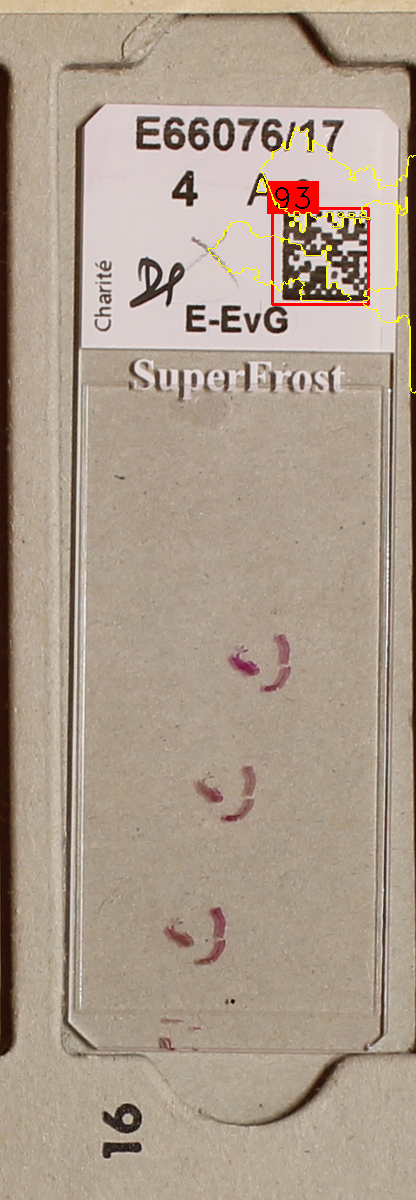
\includegraphics[width=0.2\textwidth]{./assets/Cell100325_1_6_top1_positiveonlywithrest.PNG}
      \hfill
      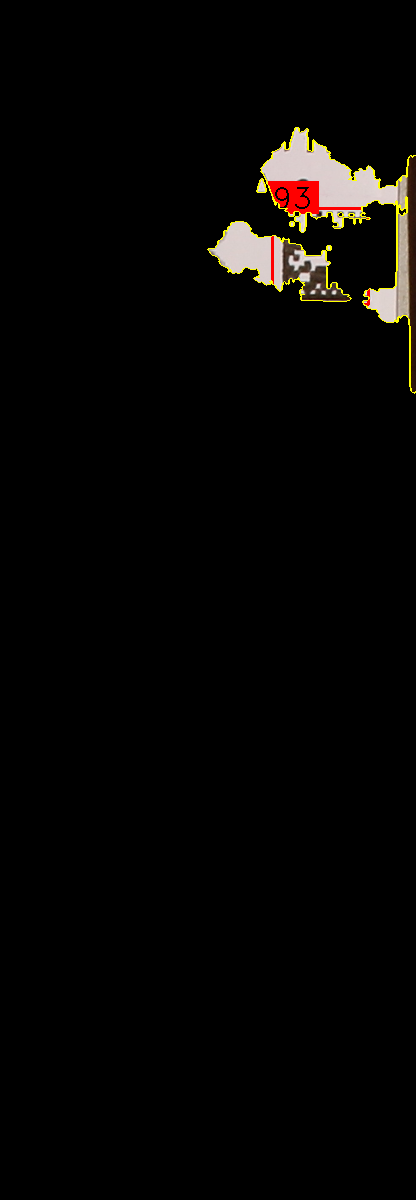
\includegraphics[width=0.2\textwidth]{./assets/Cell100325_1_6_top1_positiveonly.PNG}
      \hfill
      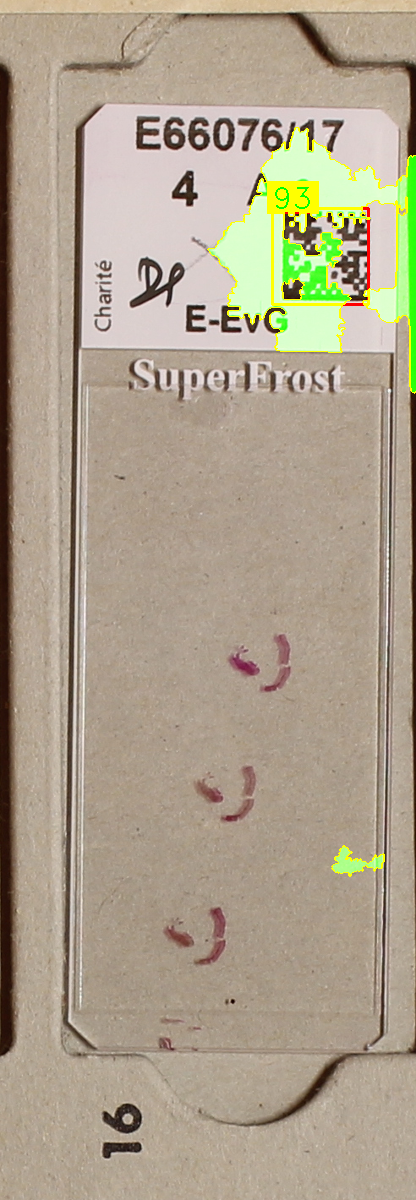
\includegraphics[width=0.2\textwidth]{./assets/Cell100325_1_6_top1_proscons.PNG}
      \hfill
      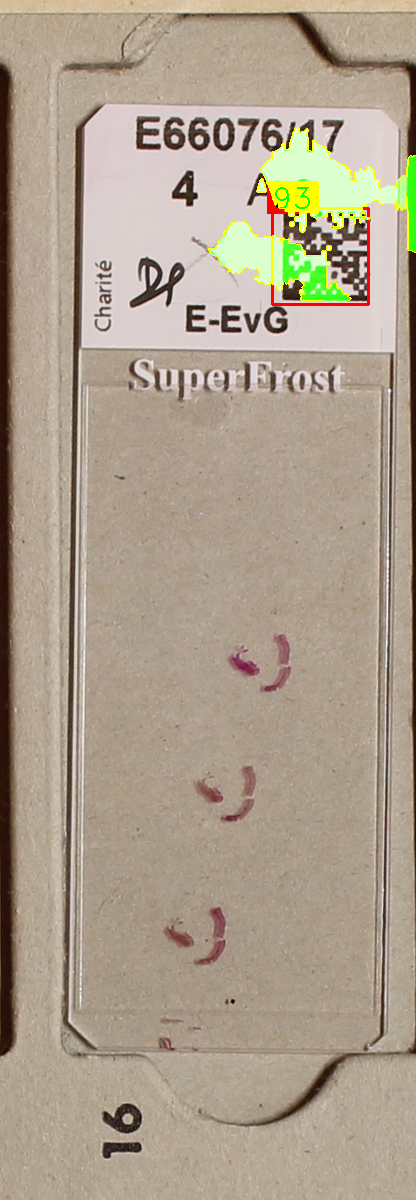
\includegraphics[width=0.2\textwidth]{./assets/Cell100325_1_6_top1_prosconsminweight.PNG}
      \caption{Data-Matrix-Code, klar gedruckter Barcode, gute Bildqualität, signiert}
    \end{figure}
  \end{frame}

  \begin{frame}{Bilder}
    \begin{figure}
      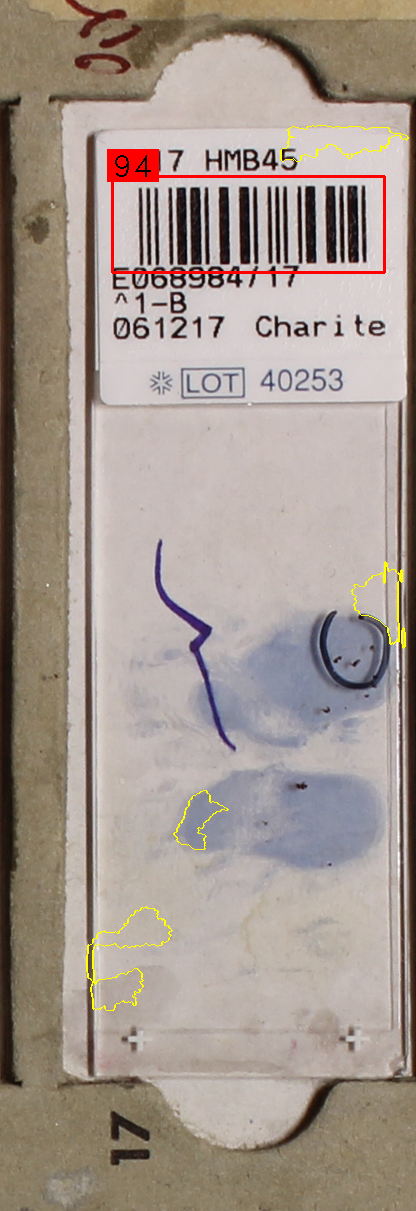
\includegraphics[width=0.2\textwidth]{./assets/Cell100426_1_7_top1_positiveonlywithrest.PNG}
      \hfill
      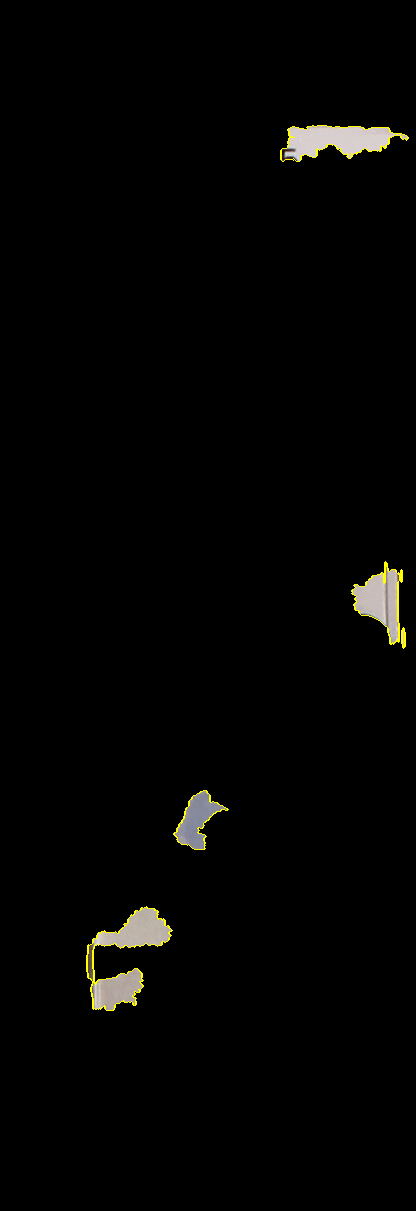
\includegraphics[width=0.2\textwidth]{./assets/Cell100426_1_7_top1_positiveonly.PNG}
      \hfill
      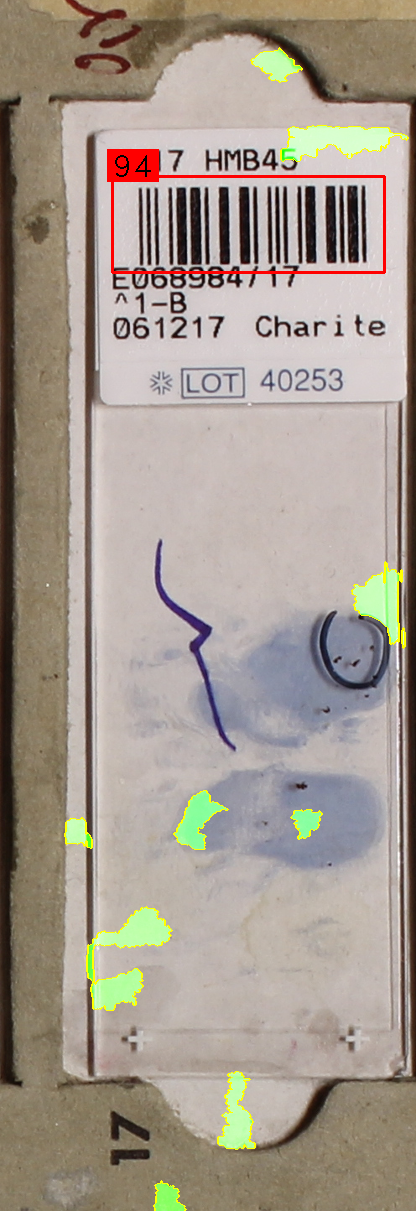
\includegraphics[width=0.2\textwidth]{./assets/Cell100426_1_7_top1_proscons.PNG}
      \hfill
      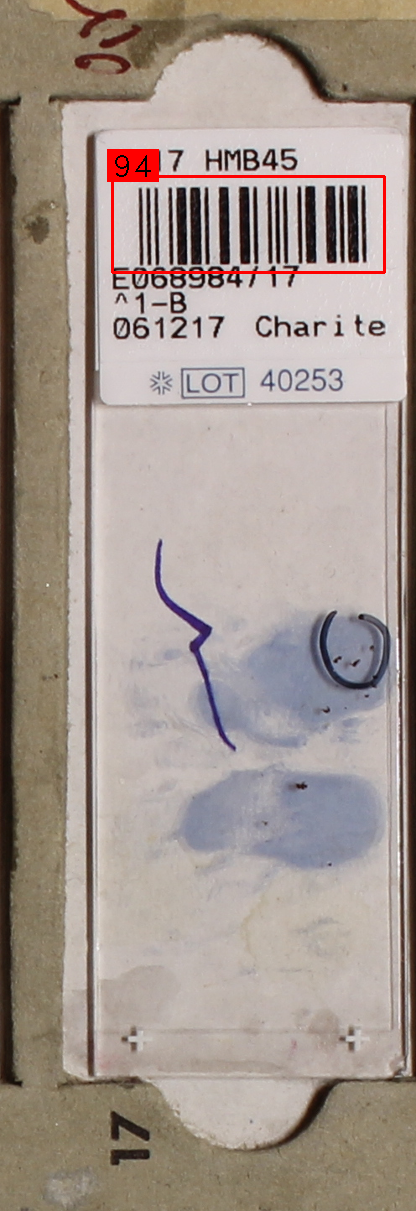
\includegraphics[width=0.2\textwidth]{./assets/Cell100426_1_7_top1_prosconsminweight.PNG}
      \caption{1D Barcode, klar gedruckter Barcode, gute Bildqualität, unsigniert}
    \end{figure}
  \end{frame}

  \begin{frame}{Bilder}
    \begin{figure}
      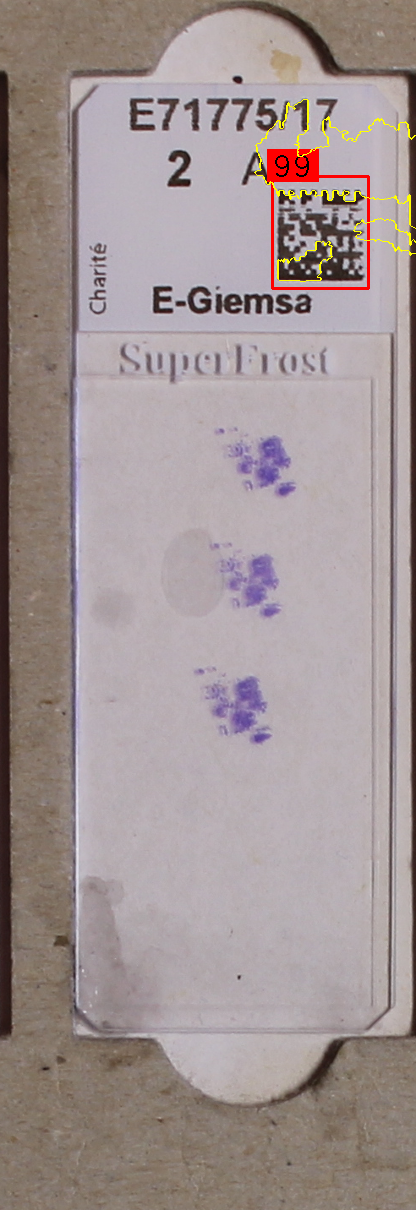
\includegraphics[width=0.2\textwidth]{./assets/Cell100884_1_5_top1_positiveonlywithrest.PNG}
      \hfill
      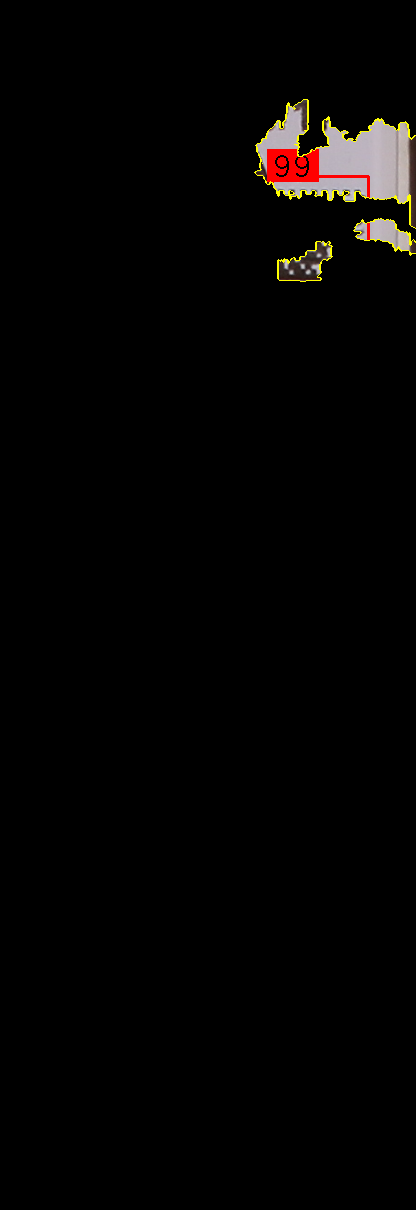
\includegraphics[width=0.2\textwidth]{./assets/Cell100884_1_5_top1_positiveonly.PNG}
      \hfill
      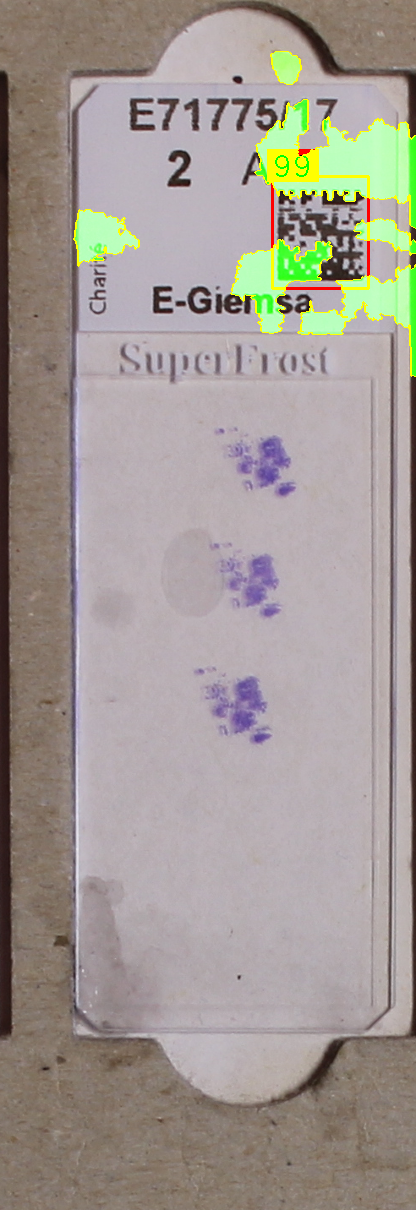
\includegraphics[width=0.2\textwidth]{./assets/Cell100884_1_5_top1_proscons.PNG}
      \hfill
      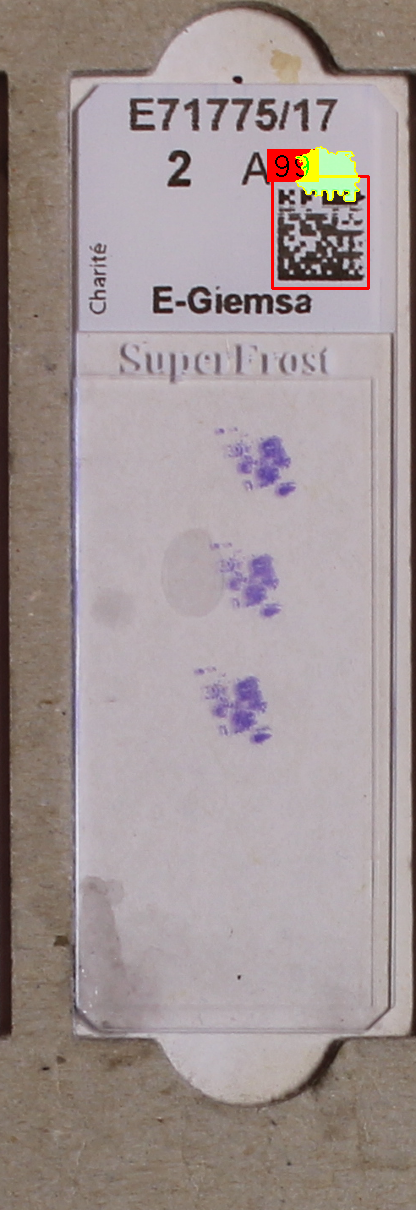
\includegraphics[width=0.2\textwidth]{./assets/Cell100884_1_5_top1_prosconsminweight.PNG}
      \caption{Data-Matrix-Code, schlechter Barcode-Druck, gute Bildqualität, unsigniert}
    \end{figure}
  \end{frame}

  \begin{frame}{Bilder}
    \begin{figure}
      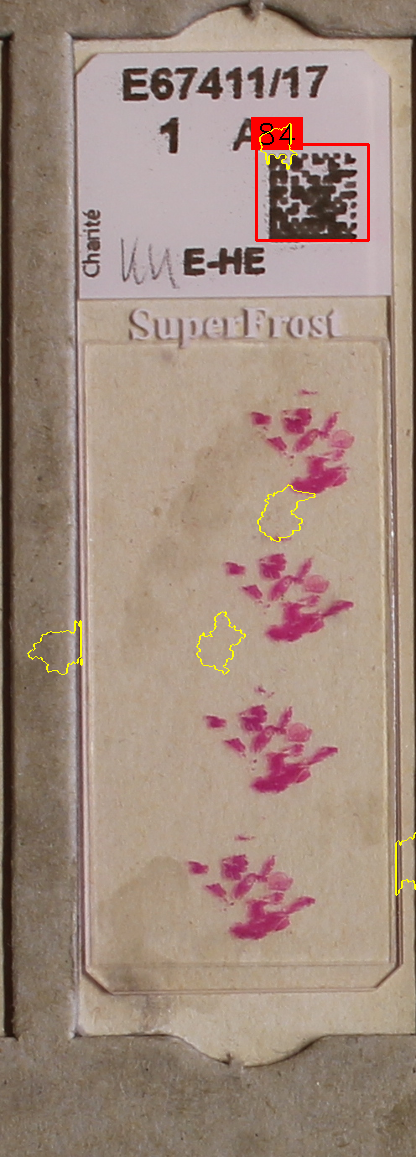
\includegraphics[width=0.2\textwidth]{./assets/Cell102723_1_4_top1_positiveonlywithrest.PNG}
      \hfill
      
\includegraphics[width=0.2\textwidth]{./assets/Cell102723_1_4_top1_positiveonly.PNG}
      \hfill
      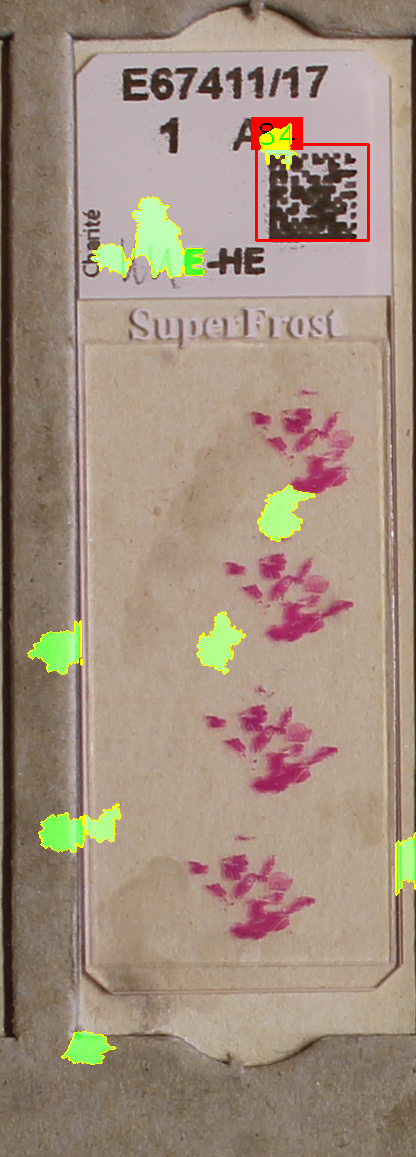
\includegraphics[width=0.2\textwidth]{./assets/Cell102723_1_4_top1_proscons.PNG}
      \hfill
      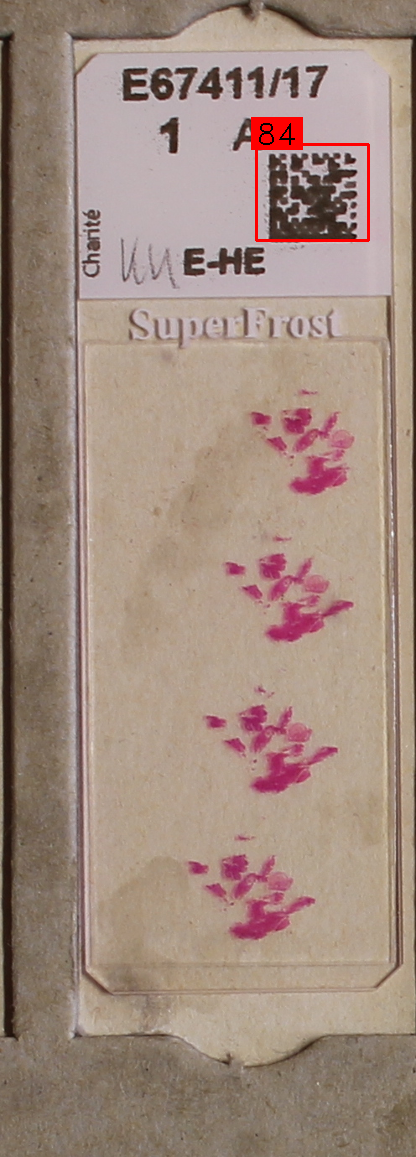
\includegraphics[width=0.2\textwidth]{./assets/Cell102723_1_4_top1_prosconsminweight.PNG}
      \caption{Data-Matrix-Code, verschwommener Barcode, gute Bildqualität, unsigniert}
    \end{figure}
  \end{frame}

  \begin{frame}{Bilder}
    \begin{figure}
      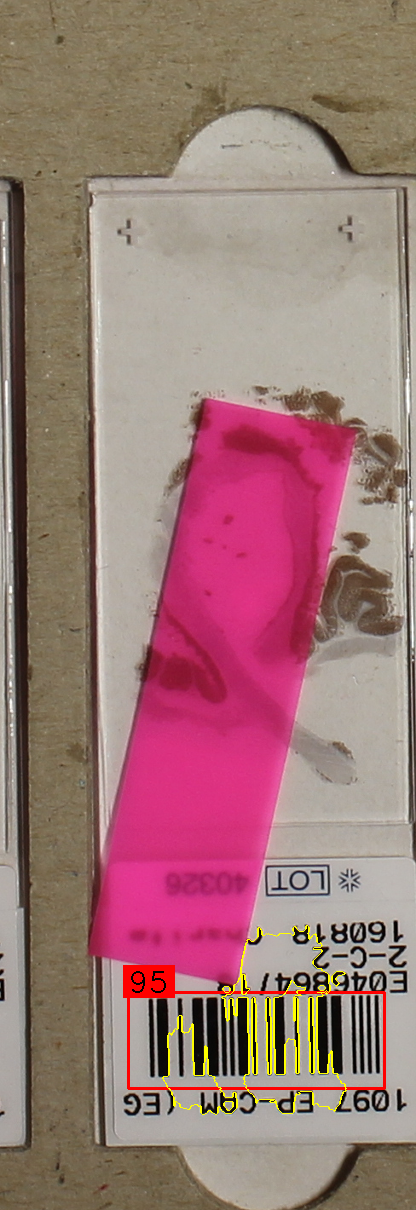
\includegraphics[width=0.2\textwidth]{./assets/Cell104473_2_4_top1_positiveonlywithrest.PNG}
      \hfill
      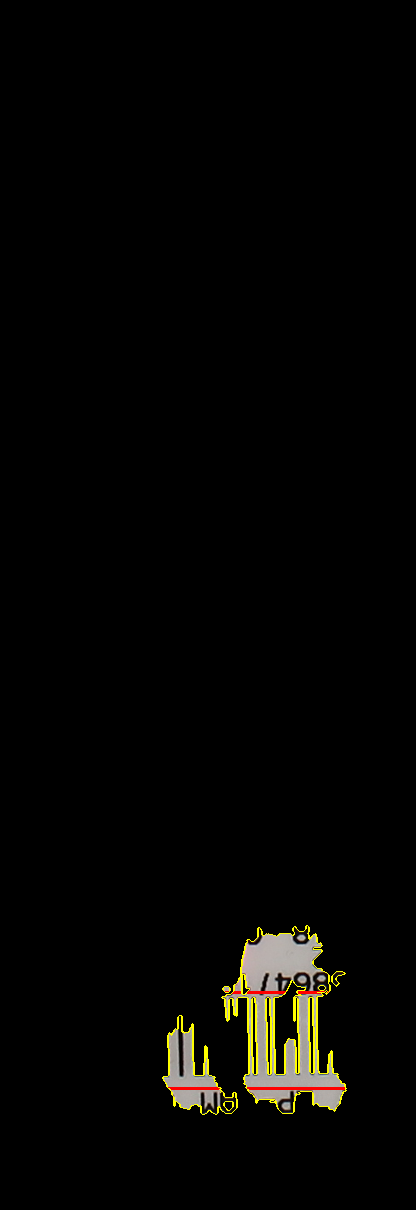
\includegraphics[width=0.2\textwidth]{./assets/Cell104473_2_4_top1_positiveonly.PNG}
      \hfill
      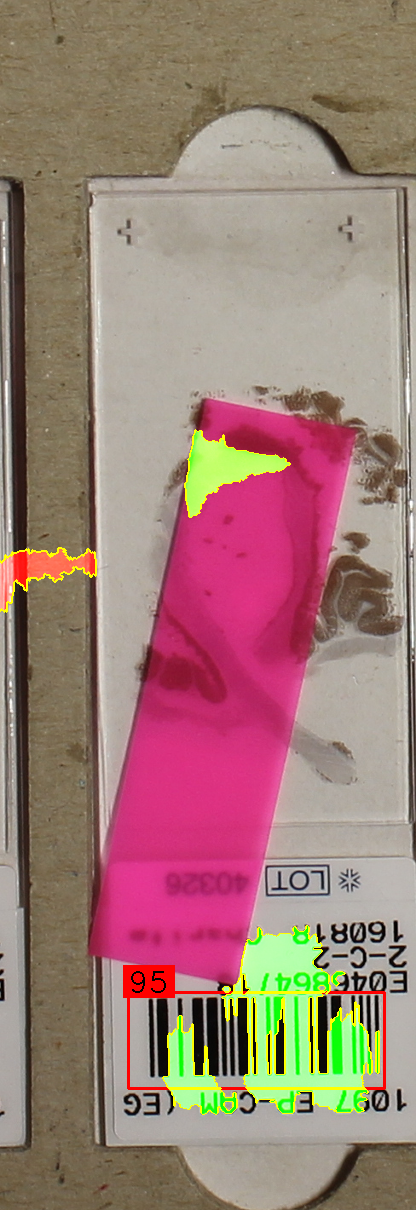
\includegraphics[width=0.2\textwidth]{./assets/Cell104473_2_4_top1_proscons.PNG}
      \hfill
      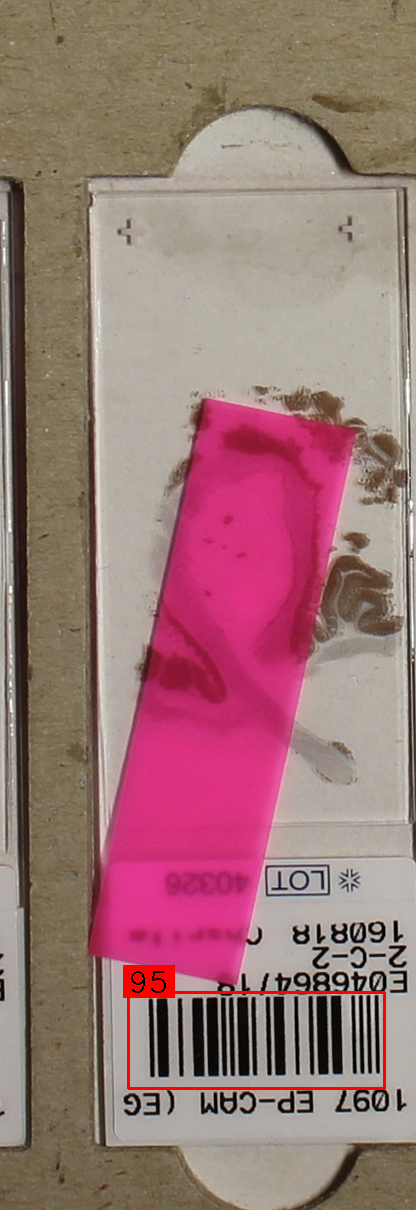
\includegraphics[width=0.2\textwidth]{./assets/Cell104473_2_4_top1_prosconsminweight.PNG}
      \caption{1D Barcode, teilweise verdeckter Barcode, gute Bildqualität, signiert}
    \end{figure}
  \end{frame}

  \begin{frame}{Bilder}
    \begin{figure}
      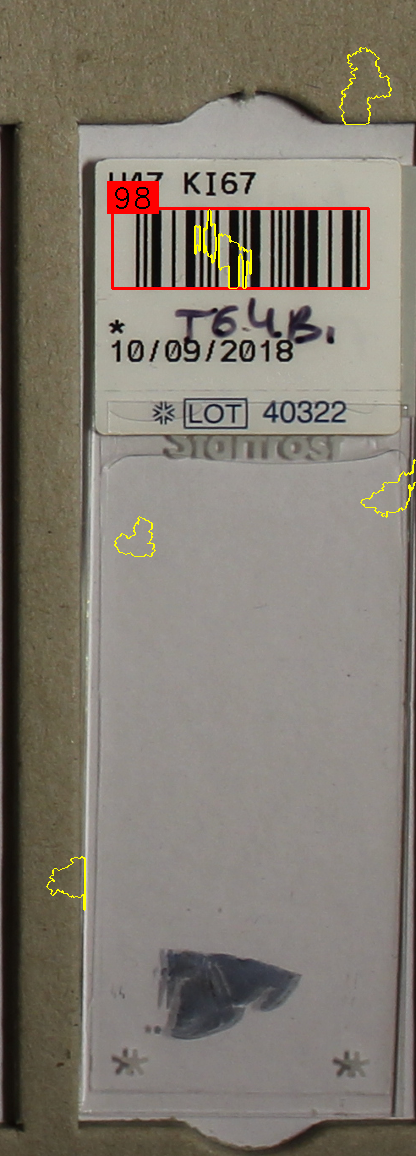
\includegraphics[width=0.2\textwidth]{./assets/Cell106357_2_8_top1_positiveonlywithrest.PNG}
      \hfill
      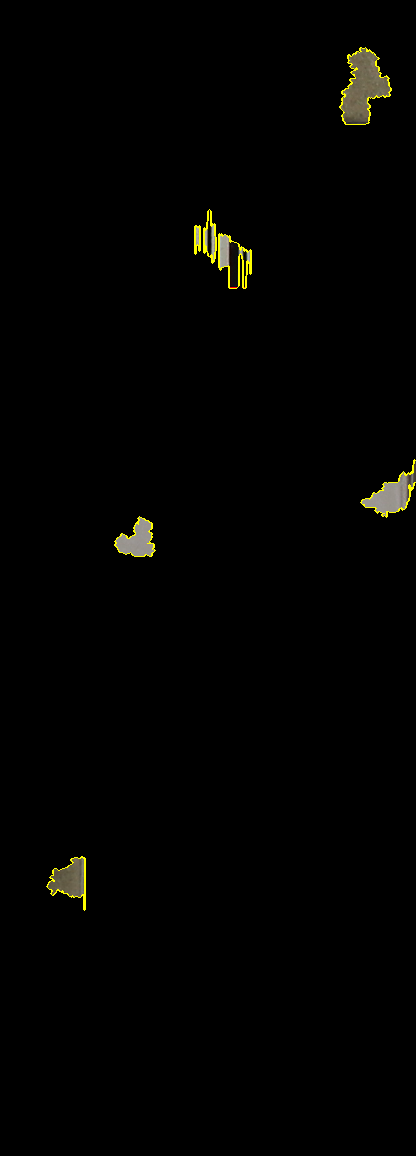
\includegraphics[width=0.2\textwidth]{./assets/Cell106357_2_8_top1_positiveonly.PNG}
      \hfill
      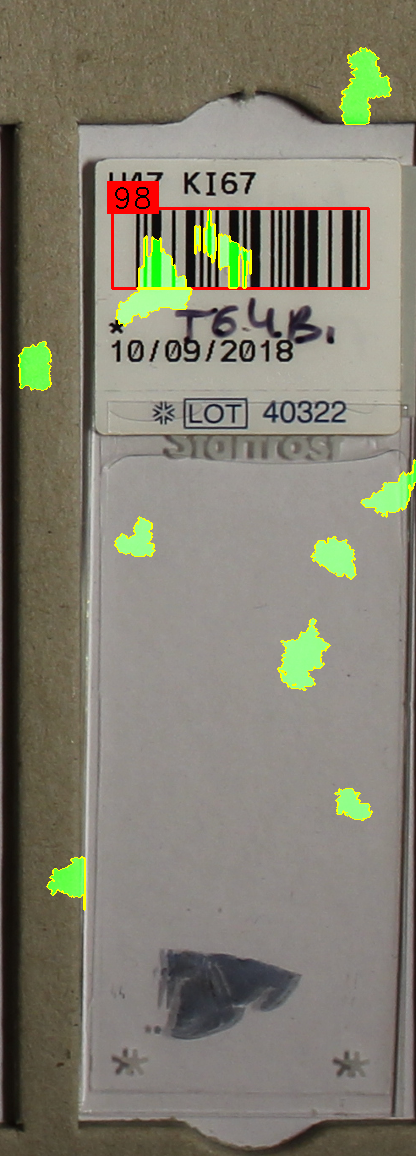
\includegraphics[width=0.2\textwidth]{./assets/Cell106357_2_8_top1_proscons.PNG}
      \hfill
      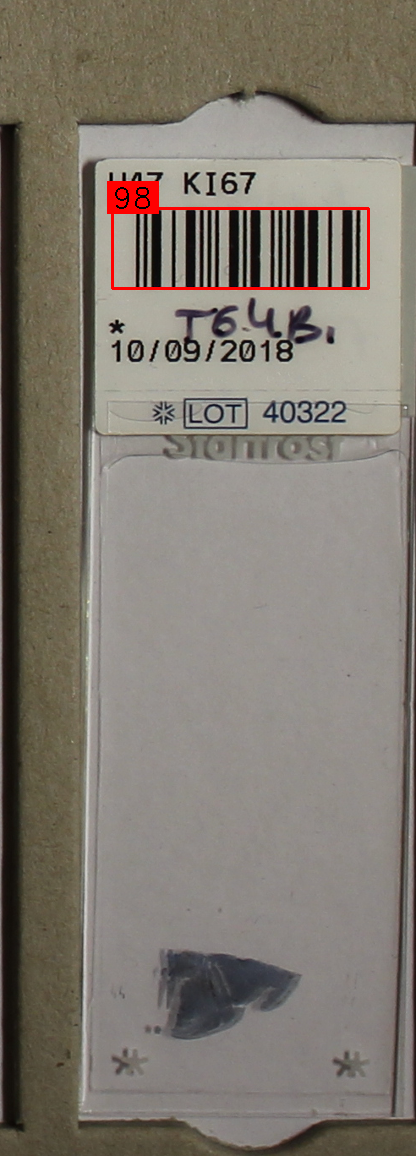
\includegraphics[width=0.2\textwidth]{./assets/Cell106357_2_8_top1_prosconsminweight.PNG}
      \caption{1D Barcode, klar gedruckter Barcode, gute Bildqualität, signiert}
    \end{figure}
  \end{frame}

  \begin{frame}{Bilder}
    \begin{figure}
      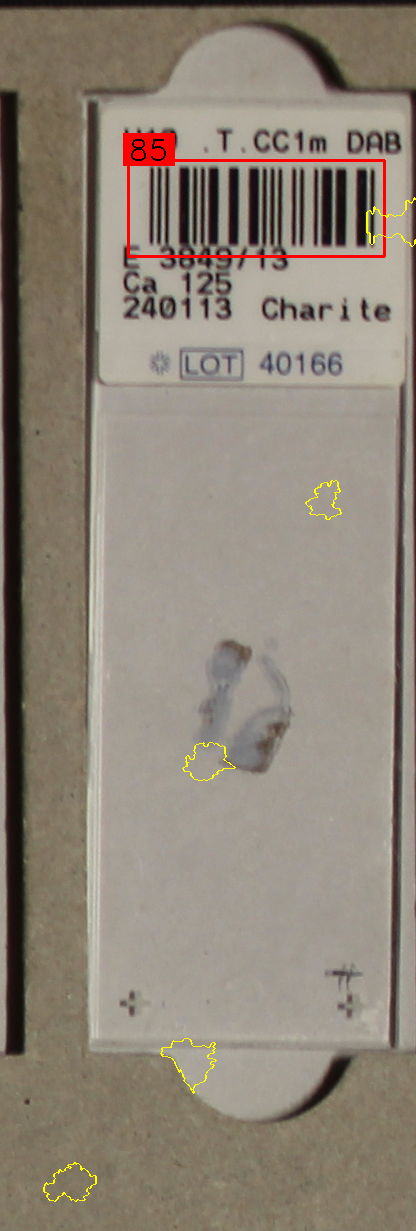
\includegraphics[width=0.2\textwidth]{./assets/Cell111308_1_9_top1_positiveonlywithrest.PNG}
      \hfill
      
\includegraphics[width=0.2\textwidth]{./assets/Cell111308_1_9_top1_positiveonly.PNG}
      \hfill
      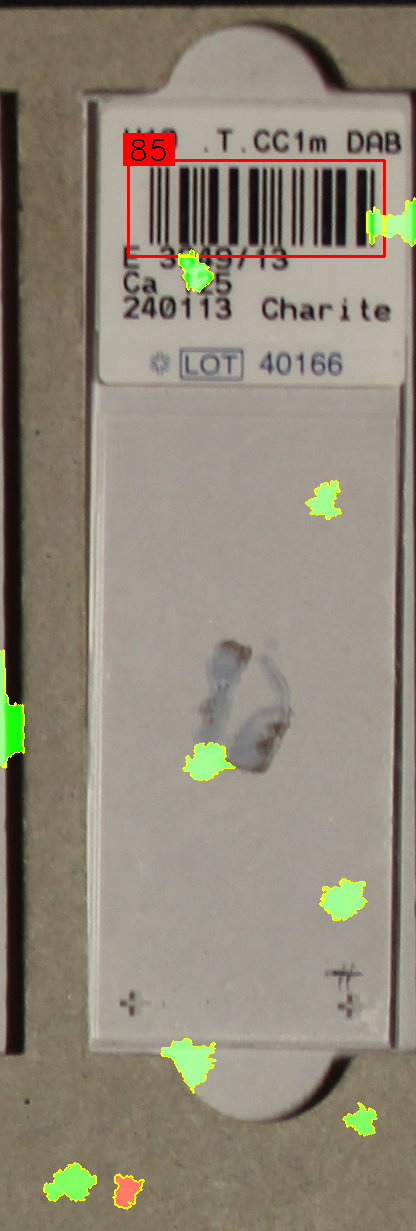
\includegraphics[width=0.2\textwidth]{./assets/Cell111308_1_9_top1_proscons.PNG}
      \hfill
      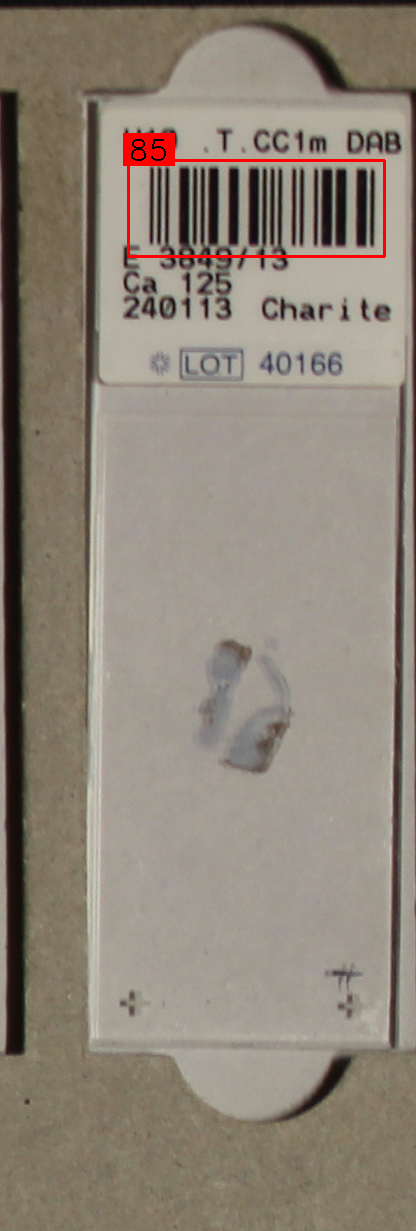
\includegraphics[width=0.2\textwidth]{./assets/Cell111308_1_9_top1_prosconsminweight.PNG}
      \caption{1D Barcode, klar gedruckter Barcode, schlechte Bildqualität, unsigniert}
    \end{figure}
  \end{frame}

  \begin{frame}{Bilder}
    \begin{figure}
      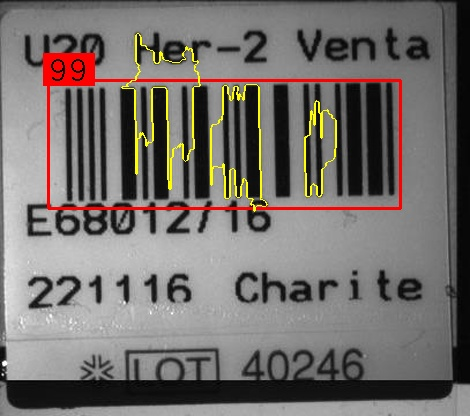
\includegraphics[width=0.2\textwidth]{./assets/E2016068012P1-A-5_GBG-Her2IH_0000000000008E5B-label_top1_positiveonlywithrest.jpg}
      \hfill
      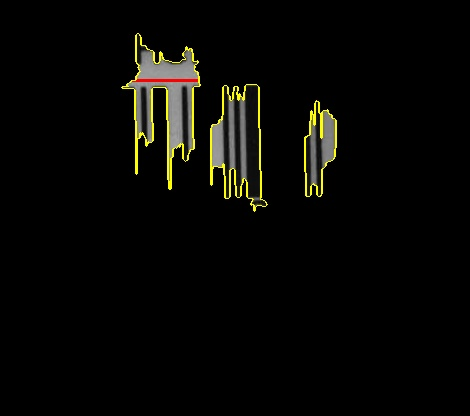
\includegraphics[width=0.2\textwidth]{./assets/E2016068012P1-A-5_GBG-Her2IH_0000000000008E5B-label_top1_positiveonly.jpg}
      \hfill
      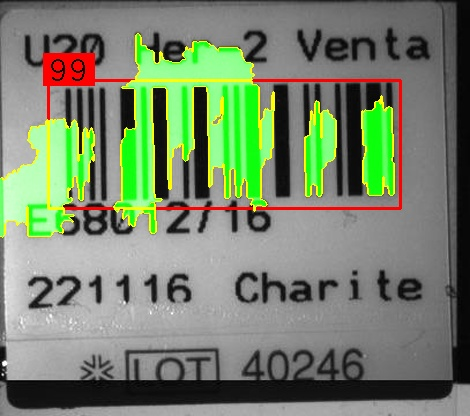
\includegraphics[width=0.2\textwidth]{./assets/E2016068012P1-A-5_GBG-Her2IH_0000000000008E5B-label_top1_proscons.jpg}
      \hfill
      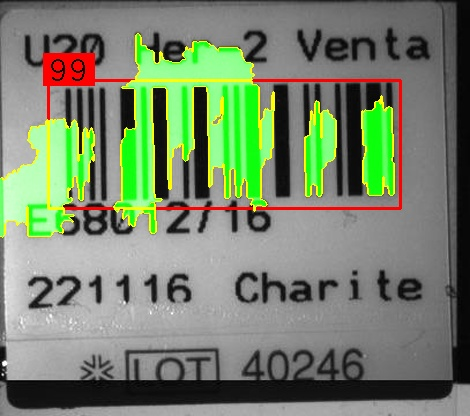
\includegraphics[width=0.2\textwidth]{./assets/E2016068012P1-A-5_GBG-Her2IH_0000000000008E5B-label_top1_prosconsminweight.jpg}
      \caption{1D Barcode, klar gedruckter Barcode, gute Bildqualität, unsigniert}
    \end{figure}
  \end{frame}

  \begin{frame}{Bilder}
    \begin{figure}
      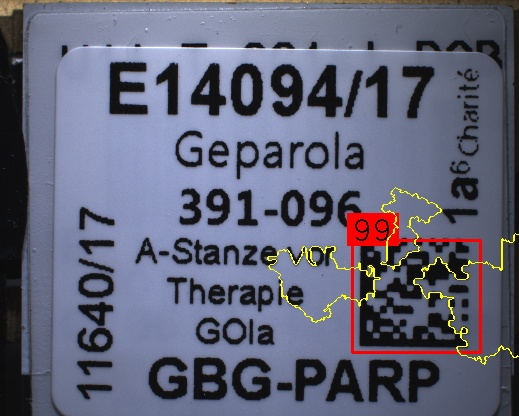
\includegraphics[width=0.2\textwidth]{./assets/E2017014094P1-a-6_GBG-PARP_0000000000009140-label_top1_positiveonlywithrest.jpg}
      \hfill
      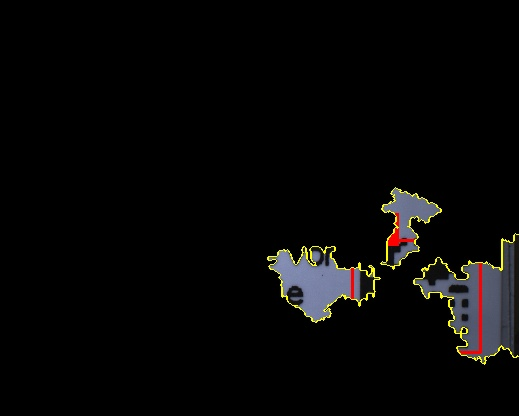
\includegraphics[width=0.2\textwidth]{./assets/E2017014094P1-a-6_GBG-PARP_0000000000009140-label_top1_positiveonly.jpg}
      \hfill
      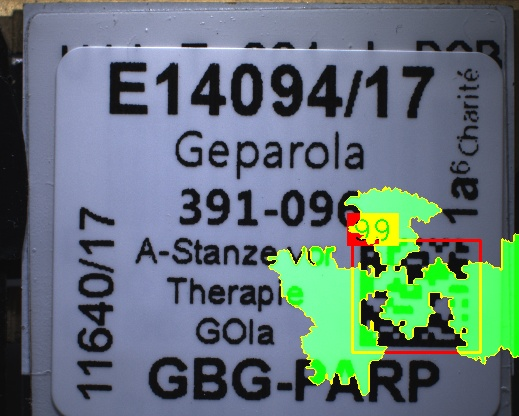
\includegraphics[width=0.2\textwidth]{./assets/E2017014094P1-a-6_GBG-PARP_0000000000009140-label_top1_proscons.jpg}
      \hfill
      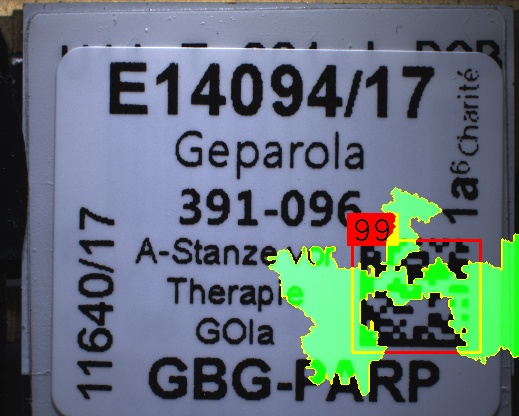
\includegraphics[width=0.2\textwidth]{./assets/E2017014094P1-a-6_GBG-PARP_0000000000009140-label_top1_prosconsminweight.jpg}
      \caption{Data-Matrix-Code, klar gedruckter Barcode, gute Bildqualität, unsigniert}
    \end{figure}
  \end{frame}

  \begin{frame}{Bilder}
    \begin{figure}
      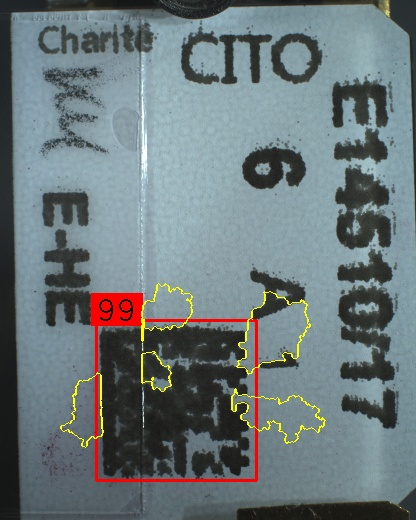
\includegraphics[width=0.2\textwidth]{./assets/E2017014510P6-A-1_E-HE_000000000000A3B3-label_top1_positiveonlywithrest.jpg}
      \hfill
      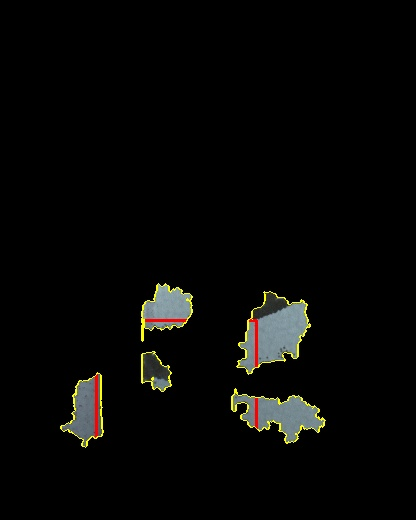
\includegraphics[width=0.2\textwidth]{./assets/E2017014510P6-A-1_E-HE_000000000000A3B3-label_top1_positiveonly.jpg}
      \hfill
      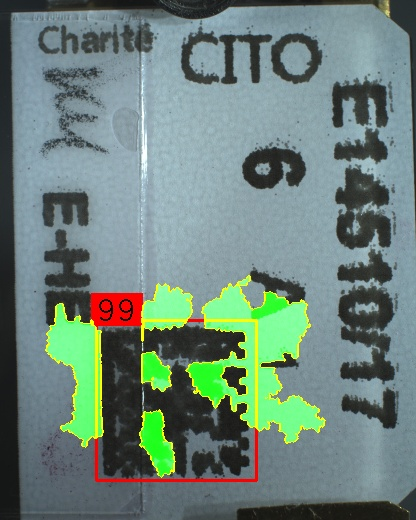
\includegraphics[width=0.2\textwidth]{./assets/E2017014510P6-A-1_E-HE_000000000000A3B3-label_top1_proscons.jpg}
      \hfill
      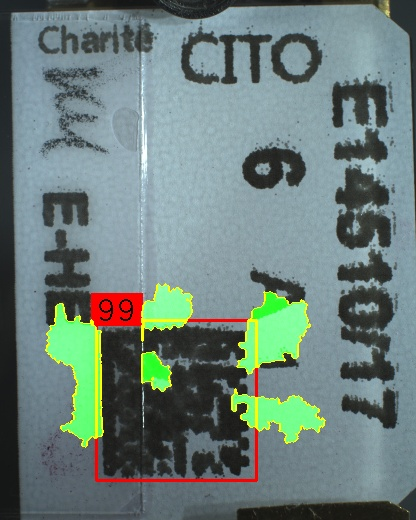
\includegraphics[width=0.2\textwidth]{./assets/E2017014510P6-A-1_E-HE_000000000000A3B3-label_top1_prosconsminweight.jpg}
      \caption{Data-Matrix-Code, verschwommener Barcode, gute Bildqualität, signiert}
    \end{figure}
  \end{frame}

  \begin{frame}{Bilder}
    \begin{figure}
      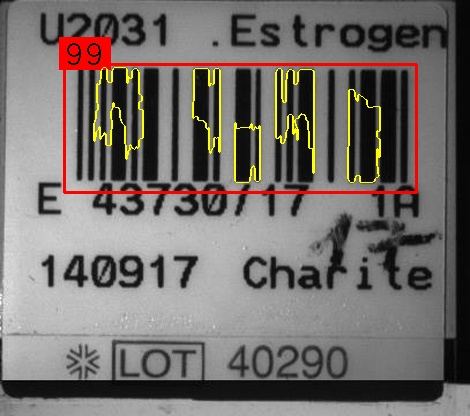
\includegraphics[width=0.2\textwidth]{./assets/E2017043730P1-A-17_IH-ER_0000000000000604-label_top1_positiveonlywithrest.jpg}
      \hfill
      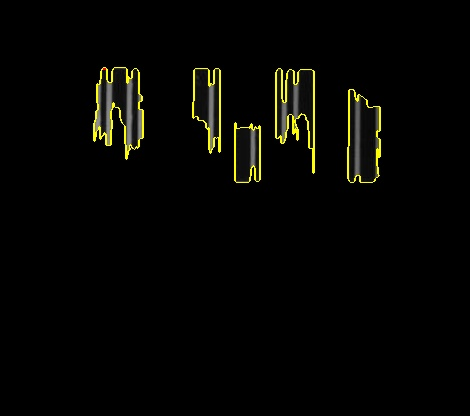
\includegraphics[width=0.2\textwidth]{./assets/E2017043730P1-A-17_IH-ER_0000000000000604-label_top1_positiveonly.jpg}
      \hfill
      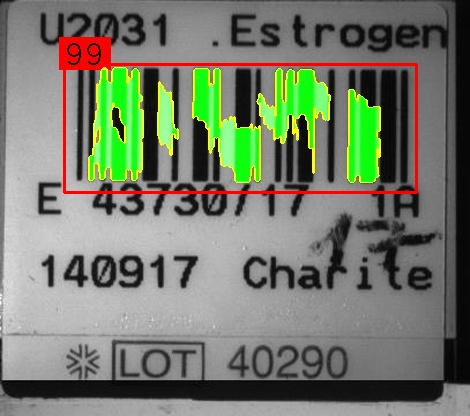
\includegraphics[width=0.2\textwidth]{./assets/E2017043730P1-A-17_IH-ER_0000000000000604-label_top1_proscons.jpg}
      \hfill
      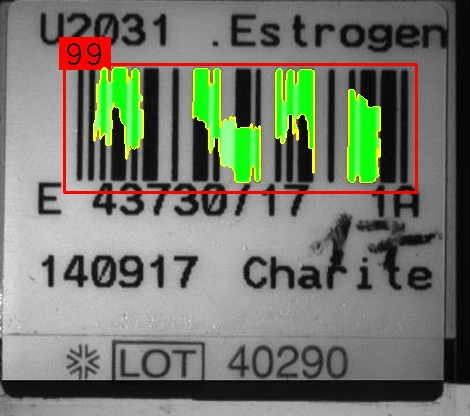
\includegraphics[width=0.2\textwidth]{./assets/E2017043730P1-A-17_IH-ER_0000000000000604-label_top1_prosconsminweight.jpg}
      \caption{1D Barcode, klar gedruckter Barcode, gute Bildqualität, signiert}
    \end{figure}
  \end{frame}

  \begin{frame}{Bilder}
    \begin{figure}
      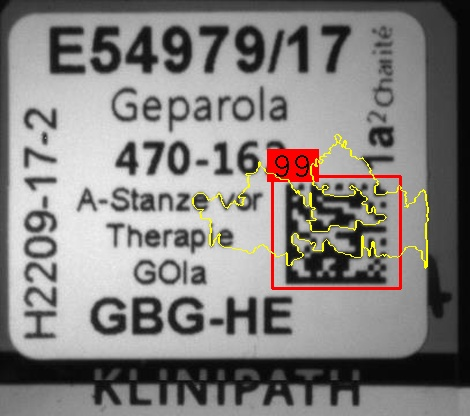
\includegraphics[width=0.2\textwidth]{./assets/E2017054979P1-a-2_GBG-HE_0000000000003162-label_top1_positiveonlywithrest.jpg}
      \hfill
      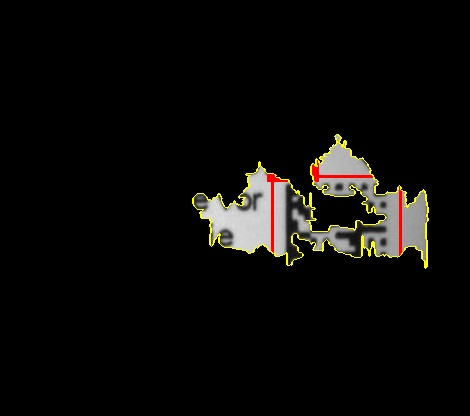
\includegraphics[width=0.2\textwidth]{./assets/E2017054979P1-a-2_GBG-HE_0000000000003162-label_top1_positiveonly.jpg}
      \hfill
      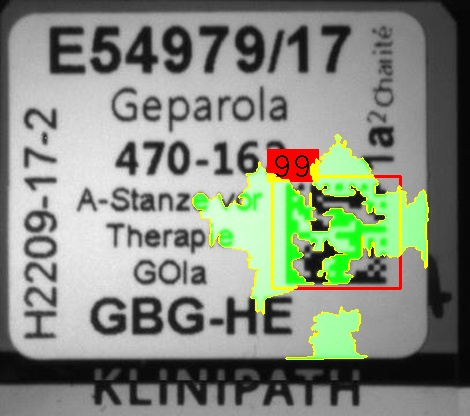
\includegraphics[width=0.2\textwidth]{./assets/E2017054979P1-a-2_GBG-HE_0000000000003162-label_top1_proscons.jpg}
      \hfill
      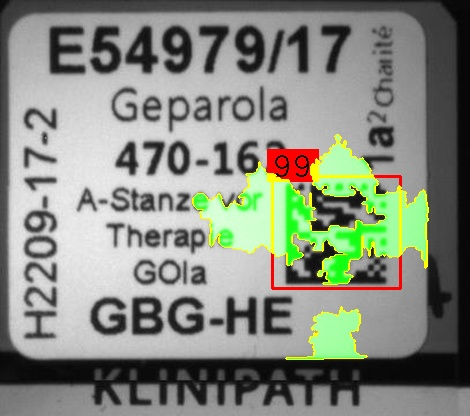
\includegraphics[width=0.2\textwidth]{./assets/E2017054979P1-a-2_GBG-HE_0000000000003162-label_top1_prosconsminweight.jpg}
      \caption{Data-Matrix-Code, klar gedruckter Barcode, schlechte Bildqualität, unsigniert}
    \end{figure}
  \end{frame}

  \begin{frame}{Bilder}
    \begin{figure}
      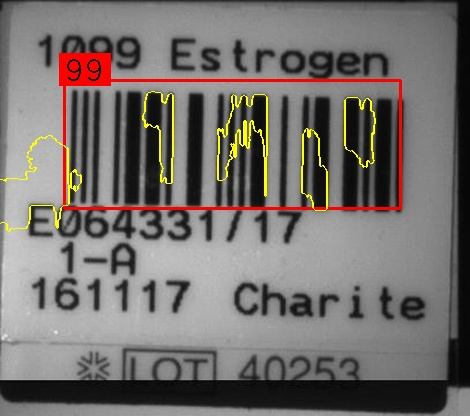
\includegraphics[width=0.2\textwidth]{./assets/E2017064331P1-A-7_IH-PR_0000000000003277-label_top1_positiveonlywithrest.jpg}
      \hfill
      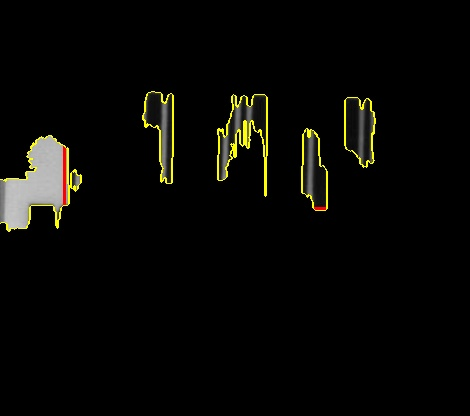
\includegraphics[width=0.2\textwidth]{./assets/E2017064331P1-A-7_IH-PR_0000000000003277-label_top1_positiveonly.jpg}
      \hfill
      \includegraphics[width=0.2\textwidth]{./assets/E2017064331P1-A-7_IH-PR_0000000000003277-label_top1_proscons.jpg}
      \hfill
      \includegraphics[width=0.2\textwidth]{./assets/E2017064331P1-A-7_IH-PR_0000000000003277-label_top1_prosconsminweight.jpg}
      \caption{1D Barcode, klar gedruckter Barcode, schlechte Bildqualität, unsigniert}
    \end{figure}
  \end{frame}

  \begin{frame}{Bilder}
    \begin{figure}
      \includegraphics[width=0.2\textwidth]{./assets/S2016000367P1-S-1_S-HE_0000000000008E83-label_top1_positiveonlywithrest.jpg}
      \hfill
      \includegraphics[width=0.2\textwidth]{./assets/S2016000367P1-S-1_S-HE_0000000000008E83-label_top1_positiveonly.jpg}
      \hfill
      \includegraphics[width=0.2\textwidth]{./assets/S2016000367P1-S-1_S-HE_0000000000008E83-label_top1_proscons.jpg}
      \hfill
      \includegraphics[width=0.2\textwidth]{./assets/S2016000367P1-S-1_S-HE_0000000000008E83-label_top1_prosconsminweight.jpg}
      \caption{Data-Matrix-Code, verschwommener und teilweise überdeckter Barcode, gute Bildqualität, unsigniert}
    \end{figure}
  \end{frame}

  \begin{frame}{Bilder}
    \begin{figure}
      \includegraphics[width=0.2\textwidth]{./assets/Cell101453_2_4_top2_positiveonlywithrest.PNG}
      \hfill
      \includegraphics[width=0.2\textwidth]{./assets/Cell101453_2_4_top2_positiveonly.PNG}
      \hfill
      \includegraphics[width=0.2\textwidth]{./assets/Cell101453_2_4_top2_proscons.PNG}
      \hfill
      \includegraphics[width=0.2\textwidth]{./assets/Cell101453_2_4_top2_prosconsminweight.PNG}
      \caption{Data-Matrix-Code \textbf{(nicht erkannt)}, klar gedruckter Barcode, gute Bildqualität, unsigniert}
    \end{figure}
  \end{frame}

  \begin{frame}[standout]
    Fragen?
  \end{frame}

  \appendix
  
  \begin{frame}[allowframebreaks]{Literatur}
    \bibliography{main}
    \bibliographystyle{plain}
  \end{frame}
  
\end{document}